%%%%%%%%%%%%%%%%%%%%%%%%%%%%%%%%%%%%%%%%%%%%%%%%%%%%%%%%%%%%%%%%%
\chapter{Operaciones Numéricas}
%%%%%%%%%%%%%%%%%%%%%%%%%%%%%%%%%%%%%%%%%%%%%%%%%%%%%%%%%%%%%%%%%

%-------------------------------------
\section{Bits, bytes y punto flotante}
%-------------------------------------
Los computadores tienen un número finito de formas de representar números. Es decir, solo pueden aproximar un pequeño subconjunto de los números reales. Comprender esto es un componente esencial para realizar operaciones numéricas: usted debe entender cómo y por qué se acumulan los errores numéricos, y cuándo interfieren con un cálculo.

La unidad de representación computacional es un \textbf{bit} (unidad representada por b), es decir, un circuito que está abierto o cerrado. Ocho bits se agrupan en un \textbf{byte} (unidad representada por B), como se muestra en la Figura \ref{fig:Byte}. Este número evolucionó a partir de las arquitecturas computacionales en los primeros días de la computación, y fue estandarizado por primera vez por la ISO/IEC 2382-1:1993. En un byte, las posiciones van de 0 a 7, usualmente representadas de derecha a izquierda. Un 1 en la primera posición representa $2^0$, en la segunda posición es $2^1$, y así sucesivamente.

\begin{figure}[h]\label{fig:Byte}
	\centering
		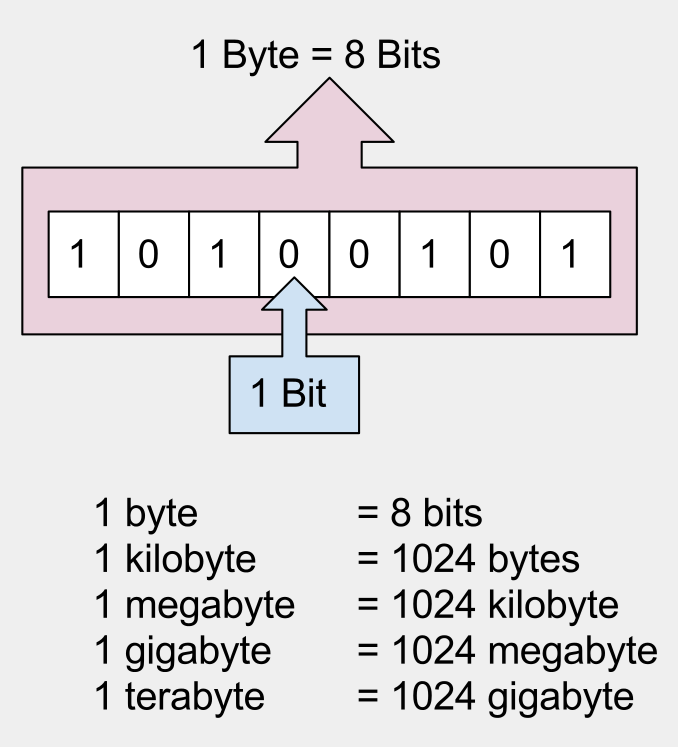
\includegraphics[width=0.5\textwidth]{../images/ChapterNumericalOps/Byte.png}
	\caption{Bits y bytes \cite{wiki:Byte}. Leyendo de izquierda a derecha, el ejemplo representa: $2^0 + 2^2 + 2^5 + 2^7 = 1 +  4 + 32 + 128= 165$. Si usted lee de derecha a izquierda (esta es la forma estándar de representar bits), obtendría $2^0 + 2^2 + 2^5 + 2^7 = 165$. En este caso, de izquierda a derecha y de derecha a izquierda producen el mismo resultado. Pero en general no tienen que ser iguales. ¿Qué ocurre si usted reemplaza algún cero por un uno y calcula de nuevo en ambas direcciones? Así, la representación importa, y usted necesita conocer la convención.}
	\label{fig:Byte}
\end{figure}

Una manera ingenua de representar números con un computador es asignar $N$ dígitos decimales para cada número. Por ejemplo:
{\ttfamily\[
	012.345
\]}
Este ejemplo representa un sistema de punto fijo de 6 dígitos. Este sistema de punto fijo de 6 dígitos produce errores en algunos casos de suma:
{\ttfamily\[
	999.999 + 999.999 = \text{DESBORDAMIENTO}
\]}
También se producen errores en la multiplicación y la división
{\ttfamily\[
	013.000 / 003.000 = 004.333
\]}
En este caso, perdemos todos los dígitos después del tercer decimal.

Podemos permitir que el punto decimal «flote» para ganar exactitud con el mismo número de dígitos. Por ejemplo:
{\ttfamily\[
	013.000 / 003.000 = 4.33333
\]}
Incluso podríamos representar números más grandes que los que 6 dígitos nos permitían antes:
{\ttfamily\[
	999.999 \times 999.999 = 9.99998 \times 10^5
\]}

%-------------------------------------
\subsection{El estándar IEEE para aritmética de punto flotante}
%-------------------------------------
El estándar IEEE para aritmética de punto flotante (IEEE 754) es un estándar técnico para el cálculo en punto flotante, establecido en 1985 por el Instituto de Ingenieros Eléctricos y Electrónicos (IEEE).
	\begin{itemize}
		\item Los números finitos pueden ser en base 2 (binario) o base 10 (decimal).
		\item Cada número finito se describe mediante tres enteros:
					\begin{enumerate}
						\item $s$ = un signo (cero o uno),
						\item $c$ = un significando (o «coeficiente»),
						\item $q$ = un exponente.
					\end{enumerate}
		\item El valor numérico de un número finito es $(-1)^s \times c \times bq$ donde b es la base (2 o 10), también llamada radix.
	\end{itemize}

Los tres campos en un flotante IEEE-754. Los números de punto flotante binarios se almacenan en una forma de signo-magnitud donde el bit más significativo es el bit de \textit{signo}, \textit{exponente} es el exponente sesgado, y \textit{fracción} es el significando menos el bit más significativo. La Figura \ref{fig:32bit} muestra un número de 32 bits, también conocido como número de punto flotante de precisión simple, mientras que la Figura \ref{fig:64bit} representa un número de 64 bits, también conocido como número de punto flotante de doble precisión.

\begin{figure}
	\centering
		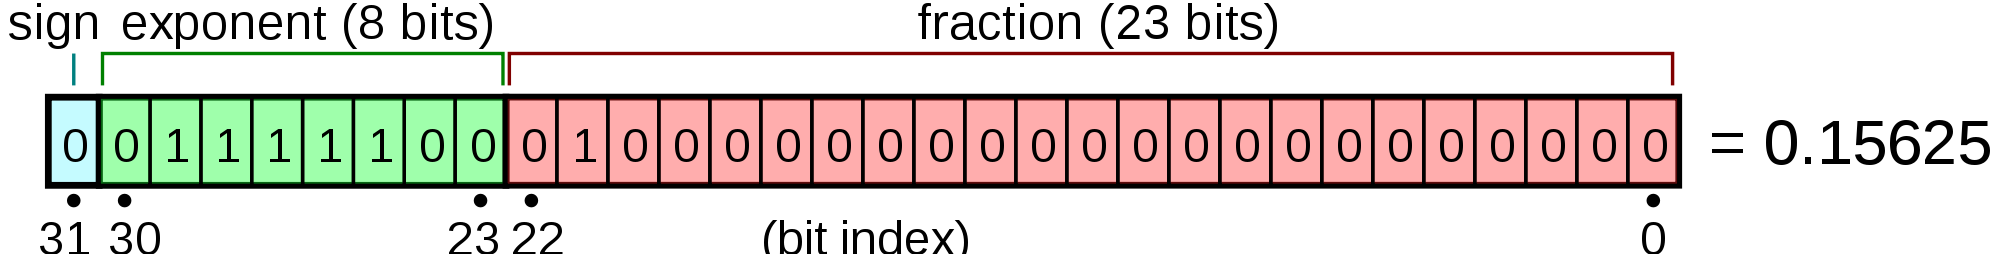
\includegraphics[width=4in]{../images/ChapterNumericalOps/Single_Floating_Point_Format.png}
		\caption{Representación de un número de precisión simple \cite{wiki:SinglePrec}}
		\label{fig:32bit}
\end{figure}

\begin{figure}
	\centering
		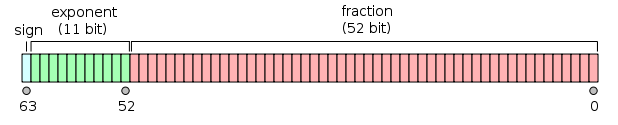
\includegraphics[width=4in]{../images/ChapterNumericalOps/Double_Floating_Point_Format.png}
		\caption{Representación de un número de doble precisión \cite{wiki:DoublePrec}.}
		\label{fig:64bit}
\end{figure}

Si queremos representar un número real con un número finito $N$ de posiciones de memoria, podemos reservar una posición para el signo, $N-k-1$ para la parte entera, y $k$ para los dígitos después del separador o parte fraccionaria. La notación adoptada convencionalmente es \cite{quarteroni2010numerical}:
\begin{equation}\label{eq:Floating}
	x = (-1)^s[a_{N-2}a_{N-3}...a_{k}.a_{k-1}a_{k-2}...a_{0}]  = (-1)^s \cdot \beta^{-k} \sum_{j=0}^{N-2}a_j \beta^j
\end{equation}
donde $\beta$ es la base de la representación (podría ser cualquier número, pero usualmente es $2$ o $10$), $s$ es 1 o 0, $N$ es el número de dígitos en el significando, $a_j$ es el $j^{th}$ dígito, $k$ es el exponente.

La representación de punto flotante en la ecuación \ref{eq:Floating} limita el número mínimo o máximo a menos que se permita algún escalamiento. En tal caso, una representación de \textit{punto flotante} está dada por
\begin{equation}\label{eq:Normalized}
	x = (-1)^s \cdot [0.a_{1}a_{2}...a_{t}] \cdot  \beta^{e} = (-1)^s \cdot m  \cdot \beta^{e-t}
\end{equation}
donde $t \in \mathbb{N}$ es el número de dígitos significativos $a_i$ con $0 \leq a_i \leq \beta - 1$, $m=a_{1}a_{2}...a_{t}$ es un número entero llamado \textit{mantisa}
con $0 \leq m \leq \beta^t-1$ y $e$ es un número entero llamado \textit{exponente} con $L \leq e \leq U$ (típicamente $L \leq 0$ y $U \geq 0$). Si exigimos $a_1 \neq 0$ y $m \geq \beta^{t-1}$ entonces la representación en la ecuación \ref{eq:Normalized} se denomina \textit{normalizada}.

%It is important to understand the context in which the word \textit{mantissa} is used.  The word \textit{mantissa} in computer science  is defined as the part of a floating-point number representing the significant digits of that number multiplied by the base raised to the exponent to give the actual value of the number; it is often used as a synonym for \textit{significand}. This, however, departs from the historical mathematical tradition because \textit{mantissa} was first defined as the part after the separator (or fractional part) of a logarithm. Thus, in mathematics, a \textit{mantissa} is the logarithm of a \textit{significand}.  }

El término \textit{mantisa} en las ciencias de la computación suele referirse a los dígitos significativos de un número de punto flotante, siendo esencialmente sinónimo de \textit{significando}. Este uso se desvía de su significado histórico en matemáticas, donde \textit{mantisa} designaba la parte fraccionaria de un logaritmo. Cabe destacar que, entre los numerosos autores que siguieron los primeros trabajos logarítmicos de John Napier, «\textit{Mirifici Logarithmorum Canonis Descriptio}» (1614) \cite{napier1614mirifici}, fue John Wallis quien utilizó la palabra «\textit{appendage}» en la versión en inglés de «\textit{A Treatise of Algebra}», \cite[p. 38]{wallis1685proposal} (1658), traducida al latín como «manti\hspace{-0.03in}$\int$\hspace{-0.06in}$\int$\hspace{-0.03in}am» (en forma moderna \textit{mantissa}) \cite[p. 41]{wallis1693opera} (1681) (véase la Figura \ref{fig:Mantissam}), para describir la parte decimal de un logaritmo, no el logaritmo de un significando. Esta distinción destaca la evolución de la terminología matemática a lo largo del tiempo.

\begin{figure}
	\centering
		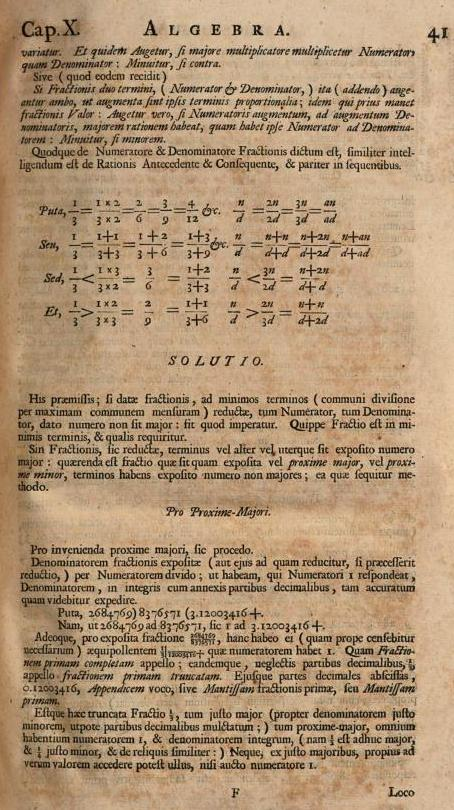
\includegraphics[width=5in]{../images/ChapterNumericalOps/Mantissam.jpg}
		\caption{Página 41 de «\textit{A Treatise of Algebra}», donde se introduce la palabra mantisa. J. Wallis. \textit{Opera mathematica: De Algebra Tractatus}. Número v. 5 Anno 1685 Anglice editus; Nunc Auctus Latine. Theatrum Sheldonianum, 1693.}
		\label{fig:Mantissam}
\end{figure}




%The total number of normalized floating point numbers of a double precision number $\mathbb{F}$ that can be represented with the IEEE standard is given by equation \ref{eq:CardinalityDouble}:
%\begin{eqnarray}
%	card \mathbb{F} & = & 2(\beta-1)\beta^{t-1}(U-L+1) + 1 \label{eq:CardinalityDouble} \\
%					& = & 2(2-1)2^{52-1}(1023-(-1022)+1) + 1 \nonumber \\
%					& = & 9.214 \times 10^{18} \nonumber
%\end{eqnarray}

%We can approximate this value by noticing that a double precision number is represented by 64 bits, starting from zero. Therefore,
%\[
%	card \mathbb{F} \approx 2^{63} \approx 9.223 \times 10^{18}
%\]

%A better approximation results invariably in equation \ref{eq:CardinalityDouble}.


%-------------------------------------
\subsection{Un bestiario de anomalías de punto flotante}\label{sec:FloatingPoint}
%-------------------------------------

Uno de los aspectos más sorprendentes de la aritmética de punto flotante es que operaciones simples no producen los resultados esperados. Por ejemplo, la suma $1-1/3-2/3$ resulta algebraicamente en cero. Sin embargo,
{\ttfamily\[
	1-1/3-2/3 = 1.1102e-16,
\]}	{\ttfamily\[
	1-2/3-1/3 = 5.5511e-17.
\]}
Así, no solo la operación no es cero, sino que además el orden de los sumandos importa, es decir, la suma en punto flotante no es conmutativa. Por lo tanto, $1-1/3-2/3 \neq 1-2/3-1/3 \neq 0$

Debido a que los números de punto flotante no pueden representar todos los números reales, se producen errores de representación en muchos casos. Pero, ¿por qué la operación no es conmutativa? \QA %Come back to this question to provide a technical answer after you read  Section \ref{sec:FloatingPoint}.

La siguiente instrucción compara si $10^{30} + 1 - 10^{30}$ es igual al valor 1. Usando aritmética elemental, la respuesta debería ser un rotundo \textit{sí}. En el lenguaje Python, el exponente se representa mediante un doble asterisco, como en Fortran, en lugar del símbolo de acento circunflejo (\^{}) usado en la mayoría de las demás plataformas de cómputo. El doble signo igual prueba si los dos lados son iguales, y devuelve un valor booleano de \textit{verdadero} o \textit{falso}. Por lo tanto, la pregunta se traduce en la siguiente instrucción:

\begin{lstlisting}[language=Python]
	10**30 + 1 - 10**30 == 1
\end{lstlisting}

Esta instrucción en particular devuelve un valor booleano de \textit{verdadero} en Python y \textit{falso} en Matlab (la sintaxis correcta de Matlab es $10\hat{\phantom{.}}30 + 1 - 10\hat{\phantom{.}}30 == 1$). Sin embargo, la siguiente sentencia:

\begin{lstlisting}[language=Python]
	10**30 + 1. - 10**30 == 1
\end{lstlisting}

\noindent devuelve \textit{falso} en Python. ¿Por qué? \QA

Una operación como

\begin{lstlisting}[language=Python]
	10**20 + 1 - 10**20 == 1
\end{lstlisting}

\noindent devuelve resultados distintos en Matlab, C, Fortran (\textit{falso}) frente a Python (\textit{verdadero}). Podría ser tentador declarar a Python el ganador en el cómputo numérico, pero lo que realmente sucede es que Python no sigue estrictamente el estándar IEEE-754. Para conocer más sutilezas del punto flotante en Python, visite \url{https://docs.python.org/3/tutorial/floatingpoint.html} En la mayoría de los casos, las desviaciones del estándar en el intérprete de Python son inofensivas y tienen un origen ideológico más que técnico. Sin embargo, es concebible que algoritmos extremos desarrollados bajo el estándar IEEE tendrían que ser adaptados cuidadosamente en Python. Existen alternativas, pero están fuera del alcance de este capítulo. Por ahora, basta decir que existen campos minados en el paisaje de Python.

Podemos explorar más discrepancias en valores extremos de punto flotante examinando en dos entornos numéricos los resultados de $10\cdot 10^b + 1 - 10\cdot 10^b$ para diferentes valores de $b$. Descargue e instale Python, Matlab, R, o compile un programa en C/C++ que ejecute las mismas operaciones. Compare lo que ocurre en estos entornos cuando elige $b \in \{10, 1e2, 1e10, 1e100, 1e1000\}$. Describa las discrepancias y analícelas. \QA



%-----------------------------------------
\section{Introducción a NumPy}
%-----------------------------------------

Para ejecutar operaciones matemáticas más allá de las operaciones básicas con números reales, usted necesita importar una biblioteca numérica. Las operaciones matriciales se ejecutan mediante funciones en NumPy. Por lo tanto, el primer paso es cargar NumPy.

\begin{lstlisting}[language=Python]
In : import numpy as np
\end{lstlisting}

La biblioteca NumPy ofrece acceso fácil a constantes de uso común, tales como:

\vs

\begin{tabular}{r|l}
Constante 			& Valor\\
\hline
np.e 				& Devuelve el número $e$ \\
np.pi 			& Devuelve el número $\pi$ \\
np.inf 			& Devuelve el número $\infty$ \\
np.nan 			& NaN, no-es-un-número \\
\hline
\end{tabular}

\vs

%MATLAB: Infinity is generated by dividing a nonzero value by zero, or by
%evaluating well defined mathematical expressions that overflow.
%(Try $10^{310}$ or $\exp(999)$.)

%MATLAB: Not-a-number is generated by trying to evaluate expressions like
%0/0 or Inf-Inf that do not have well defined mathematical values.

Con NumPy, ahora podemos acceder a funciones matemáticas de uso común. Entre otras: \vs

\begin{tabular}{r|l}
Función 			& Operación \\
\hline
np.abs(x)   		& Valor absoluto $|x|$ \\
np.sqrt(x)			&  Raíz cuadrada $\sqrt{x}$ \\
np.exp(x) 			& Función exponencial $e^x$ \\
np.log(x) 			& $\log(x)$ donde $x$ es un número real positivo\\
np.sin(x)			&  $\sin(x)$ donde se asume que $x$ está en radianes \\
np.cos(x) 			& $\cos(x)$ donde se asume que $x$ está en radianes \\
\hline
\end{tabular}

\vs
Las expresiones usan los operadores aritméticos y las reglas de precedencia que usted ya conoce a estas alturas.
También hay funciones, como coseno o seno. Usted rodea la
entrada de la función con paréntesis. Por ejemplo, para calcular la
raíz cuadrada de dos, se escribe

\begin{lstlisting}[language=Python]
In 	: np.sqrt(2)
Out	: 1.4142135623730951
\end{lstlisting}

Sin embargo, usted no puede usar la función {\s sqrt} con números negativos. ¿Qué tendría que hacer para permitir a Python calcular la raíz cuadrada de un número negativo y devolver un número complejo? \QA  %So, instead of {\s sqrt(-2)} you will have to use {\s (-2)**0.5}.

La biblioteca NumPy tiene \textit{muchas} funciones. Se puede encontrar una lista exhaustiva en \url{https://numpy.org/doc/stable/reference/}. Usted observará que inmediatamente debajo del comando que ingresó, la indicación mostrará {\s Out[n]: 3.0}, donde {\s n} representa el número de secuencia del comando (recuerde, el primer comando ejecutado tiene $n=1$, el segundo $n=2$, y así sucesivamente).

Ahora ingrese el siguiente comando:

\begin{lstlisting}[language=Python]
	x = np.random.standard_normal(3)
\end{lstlisting}

No hay salida. ¿Por qué piensa usted que este es el comportamiento? \QA En el lado derecho de la ventana de Spyder hay una pestaña llamada \textit{Variable Explorer}. Mostrará el valor de $x$. Alternativamente, usted puede ingresar

\begin{lstlisting}[language=Python]
	print(x)
\end{lstlisting}

Alternativamente, usted puede imprimir el resultado directamente sin asignarlo a una variable. Pruebe

\begin{lstlisting}[language=Python]
	print(np.random.standard_normal(3))
\end{lstlisting}

¿Por qué los resultados de esta última operación son diferentes a los valores almacenados en la variable $x$? \QA



%-----------------------------------------
\subsection{Operaciones matriciales}
%-----------------------------------------

El elemento de datos básico en NumPy es un arreglo multidimensional.
A veces se atribuye un significado especial a las matrices de 1 por 1, que se
denominan escalares, y a las matrices con una sola fila o columna, que
se denominan vectores. Python tiene otras maneras de almacenar datos tanto numéricos
como no numéricos, pero al principio es usualmente mejor
pensar en todo como una matriz.

Los vectores fila se delimitan en la notación con corchetes. Una coma separa los números individuales en un vector fila. Múltiples vectores fila del mismo tamaño se separan por comas, y se delimitan con corchetes para definir una matriz. Es una práctica común usar una letra mayúscula al nombrar matrices para distinguirlas de un vector único, escalar o valor de variable.

Ahora, crearemos un vector y una matriz para demostrar operaciones matriciales simples \vs

\begin{tabular}{r|l}
Función 			& Operación \\
\hline
$x = np.array([1,2,3,4])$ 					&   Crea el vector fila $\x = [1,2,3,4]$\\
$b = np.array([1,2,3])$ 					&   Crea el vector fila $\bb = [1,2,3]$\\
$A = np.array([[1,2,3], [4,5,6], [7,8,9]])$  &   Crea la matriz $ A = \begin{bmatrix} 1 & 2 & 3\\ 4 & 5 & 6 \\ 7 & 8 & 9 \end{bmatrix} $\\
$B = np.ones([2,3])$   &   Crea la matriz $ A = \begin{bmatrix} 1 & 1 & 1\\ 1 & 1 & 1 \end{bmatrix} $\\
$C = np.zeros([2,3])$   &   Crea la matriz $ A = \begin{bmatrix} 0 & 0 & 0\\ 0 & 0 & 0 \end{bmatrix} $\\
\hline
\end{tabular}

\vs
Los siguientes comandos demuestran casos básicos de manipulación de vectores:
\vs

\begin{tabular}{r|l}
Operación 			& Resultado \\
\hline
$x[-1]$ 				&   Devuelve 4, el último elemento de $x$\\
$x[1]$ 					&   Devuelve 2, el segundo elemento de $x$\\
$x[-2]$ 				&  Devuelve 3, el penúltimo elemento de $x$\\
\hline
\end{tabular}

\vs
El operador de dos puntos (:) es notable. En notación vectorial, indica un rango de filas o columnas. En Python, el primer elemento de un vector tiene índice 0; el segundo elemento tiene índice 1, y así sucesivamente. El operador de dos puntos $a:b$ comienza en la fila o columna de índice $a$ y cubre hasta un índice menor que $b$. Así, $A[0:2,0:2]$ devuelve una matriz compuesta por las filas 1 a 2 y las columnas 1 a 2 con respecto a la matriz $A$.

Los siguientes comandos demuestran casos básicos de manipulación de matrices:
\vs

\begin{tabular}{r|l}
Operación 			& Resultado \\
\hline
$A[1,2]$ 				&  Valor de la $2^{st}$ fila y $3^{nd}$ columna de $A$\\
$A[0:2,0:2]$ 		&  Devuelve $A = \begin{bmatrix} 1 & 2 \\ 4 & 5\end{bmatrix} $\\
$A[1:3,1:3]$ 		&  Devuelve $A = \begin{bmatrix} 5 & 6 \\ 8 & 9\end{bmatrix} $\\
%$A[1:100,1:100]$ 		&  Returns $A = \begin{bmatrix} 5 & 6 \\ 8 & 9\end{bmatrix} $\\
\hline
\end{tabular}

\vs

La matriz $A$ tiene tres filas y tres columnas. Entonces, ¿por qué $A[1:100,1:100]$ no produce un error? \QA

El tamaño o dimensión de una matriz se refiere al número de filas y
al número de columnas que tiene una matriz. El comando {\s shape} devuelve el número
de filas y columnas de una matriz.
Observe que el resultado es un vector: una matriz unidimensional con
2 valores donde el primero es el número de filas y el segundo valor
es el número de columnas. Al acceder a cada elemento de este vector,
podemos acceder a cada dimensión individualmente.

Usando la matriz $A$ de nuestros ejemplos anteriores,

\begin{lstlisting}[language=Python]
In 	: y = A.shape()
In 	: y
Out : (3,3)
In 	: y[0]
Out : 3
In 	: y[1]
Out : 3
\end{lstlisting}

El siguiente ejemplo ilustrará una sutileza al copiar matrices:

\begin{lstlisting}[language=Python]
In 	: D = A
Out :
array([[1, 2, 3],
       [4, 5, 6],
       [7, 8, 9]])
In 	: D[0,0] = 9
In 	: A
Out :
array([[9, 2, 3],
       [4, 5, 6],
       [7, 8, 9]])
\end{lstlisting}

Observe que al actualizar un valor en $D$, el valor correspondiente en $A$ cambió. ¿Por qué? ¿Qué necesitaría hacer para evitar que una actualización en $D$ modifique a $A$? \QA

Las operaciones matriciales básicas se listan a continuación, usando las matrices de los ejemplos anteriores.
\vs

\begin{tabular}{r|l}
Operación 		& Resultado \\
\hline
$A.T$ 	&  Transpuesta de $A$.\\
$A.conj().T$ 	&  Transpuesta conjugada de $A$.\\
$A@B.T$ 			&  Multiplicación matricial $A \cdot B$. \\
$A\star A$ 		&  Multiplicación elemento a elemento\\
$A/A$ 		&  División elemento a elemento\\
$A\star\star 2$ 		&  Exponenciación elemento a elemento\\
\hline
\end{tabular}

\vs

NumPy ofrece una forma fácil de resolver sistemas de ecuaciones lineales. Dada la matriz $A$ y el vector $\bb$ de los ejemplos anteriores, el sistema lineal $A\x = \bb$ se puede resolver invocando {\s np.linalg.solve} de la siguiente manera

\begin{lstlisting}[language=Python]
In 	: x = np.linalg.solve(A,b)
Out : array([-0.23333333,  0.46666667,  0.1       ])
\end{lstlisting}

Es fácil usar la multiplicación matricial $A\x$ para verificar la respuesta

\begin{lstlisting}[language=Python]
In 	: A@x
Out : array([1., 2., 3.])
\end{lstlisting}


%-----------------------------------------
\section{Tareas específicas para este laboratorio}
%-----------------------------------------
El siguiente capítulo es una clase sobre el análisis de componentes principales (PCA, por sus siglas en inglés), una de las técnicas más básicas para el análisis de datos. Implemente un análisis de componentes principales de acuerdo con el siguiente procedimiento (use NumPy para realizar las operaciones matriciales):

\begin{enumerate}
	\item Seleccione el peso al nacer junto con otras variables numéricas del conjunto de datos NCHS. Llamaremos a esto la \textit{matriz de características}.
	\item Asegúrese de que la media sea cero para cada variable. ¿Cómo logra esto? \QA Llamaremos a esto la \textit{matriz de características normalizada}.
	\item Calcule el producto interno de la matriz de características normalizada. ¿Cuál es la dimensión de la matriz resultante? \QA
	\item Calcule los valores propios y los vectores propios para el producto interno de la matriz de características normalizada. Necesitará ordenar los valores propios por magnitud. ¿Cómo hace esto en Python? \QA
	\item Proyecte los datos de la matriz de características a lo largo de los vectores propios correspondientes a los dos valores propios más grandes. Grafique cada observación en este espacio proyectado según el cuartil del peso al nacer. Es posible que necesite elegir diferentes variables hasta que surja un patrón aproximado. Interprete la gráfica. \QA
\end{enumerate}

Observe que no se espera que usted simplemente llame a una biblioteca de PCA.

%\bibliographystyle{abbrv}
%\bibliography{DocBibliography}
%\printbibliography

